\section{Projeto}

Este projeto foi inicialmente desenvolvido como parte da disciplina MC970, que estou cursando neste semestre. O objetivo principal do programa é gerar imagens de fractais, um processo que exige um número elevado de iterações para alcançar um nível considerável de detalhe e permitir a percepção das características intrínsecas dessas estruturas. Devido à natureza altamente paralelizável do problema, a implementação em linguagens como C ou CUDA é ideal. No entanto, optou-se por não desenvolver uma versão em CUDA para evitar dificuldades na execução em diferentes ambientes.

\subsection{Motivação da Escolha da Linguagem}

Embora a linguagem Python pudesse ser utilizada para implementar o projeto, sua escolha seria ineficiente para este tipo de aplicação. Python, sendo uma linguagem interpretada e de alto nível, apresenta desempenho inferior em comparação com C para operações intensivas em processamento, como o cálculo de fractais. Além disso, o gerenciamento de threads em Python é limitado pelo Global Interpreter Lock (GIL), o que restringe a execução paralela em múltiplos núcleos de CPU. Assim, a escolha de C foi mais adequada para garantir eficiência e desempenho.

Embora a linguagem CUDA fosse uma alternativa para execução altamente paralela na GPU, sua adoção implicaria em dependências de hardware (placas compatíveis com NVIDIA CUDA), além de limitar a portabilidade e aumentar a complexidade da depuração e desenvolvimento. Assim, optou-se por manter a implementação em C, permitindo execução em qualquer sistema com suporte a threads POSIX.

\subsection{Definições e Flags de Execução}

A estrutura para tratamento de parâmetros via linha de comando utiliza a biblioteca \texttt{getopt\_long}. As opções disponíveis estão descritas a seguir:


\begin{lstlisting}[caption=Flags de linha de comando]
static struct option long_options[] = {
    {"threads", required_argument, 0, 't'},
    {"help", no_argument, 0, '?'},
};
\end{lstlisting}


\subsection{Constantes e Domínio do Problema}

A resolução e a área do plano complexo são definidas pelas seguintes constantes:

\begin{lstlisting}[caption=Constantes principais]
const unsigned int scale = 2;
const unsigned int width = 7680 * scale;
const unsigned int height = 4320 * scale;
const int maxIterations = 10000;
int numThreads = 8;

float x0 = -2;
float x1 = 1;
float y0 = -1;
float y1 = 1;
\end{lstlisting}

\subsection{Resolução da Imagem}

A resolução foi fixada em \( 15360 \times 8640 \), o que corresponde a uma qualidade 16K. Tal definição visa garantir a visualização detalhada da fronteira do conjunto de Mandelbrot, onde os padrões complexos são mais interessantes e exigem alta densidade de pixels para serem adequadamente renderizados.

\subsection{Número Máximo de Iterações}

O número máximo de iterações foi definido como \( 10.000 \). Esse valor foi escolhido para detalhar ainda mais as características intrínsecas do conjunto de Mandelbrot, permitindo a visualização precisa das estruturas complexas e padrões que emergem nas regiões de fronteira. Um número elevado de iterações é essencial para capturar os detalhes mais sutis, especialmente em áreas onde a convergência é mais lenta.

\subsection{Comparação de Imagens com Diferentes Iterações}

Para ilustrar o impacto do número de iterações no nível de detalhe das imagens geradas, foram produzidas duas imagens do conjunto de Mandelbrot. A primeira foi gerada com \( 10.000 \) iterações, enquanto a segunda utilizou apenas \( 50 \) iterações. Ambas as imagens estão apresentadas abaixo para comparação:
\begin{figure}[H]
    \centering
    \begin{minipage}{0.49\textwidth}
        \centering
        
\includegraphics[width=\textwidth]{figures/comparacao/mandelbrot_10000.png}
        \caption*{Imagem com 10.000 iterações}
    \end{minipage}
    \hfill
    \begin{minipage}{0.49\textwidth}
        \centering
        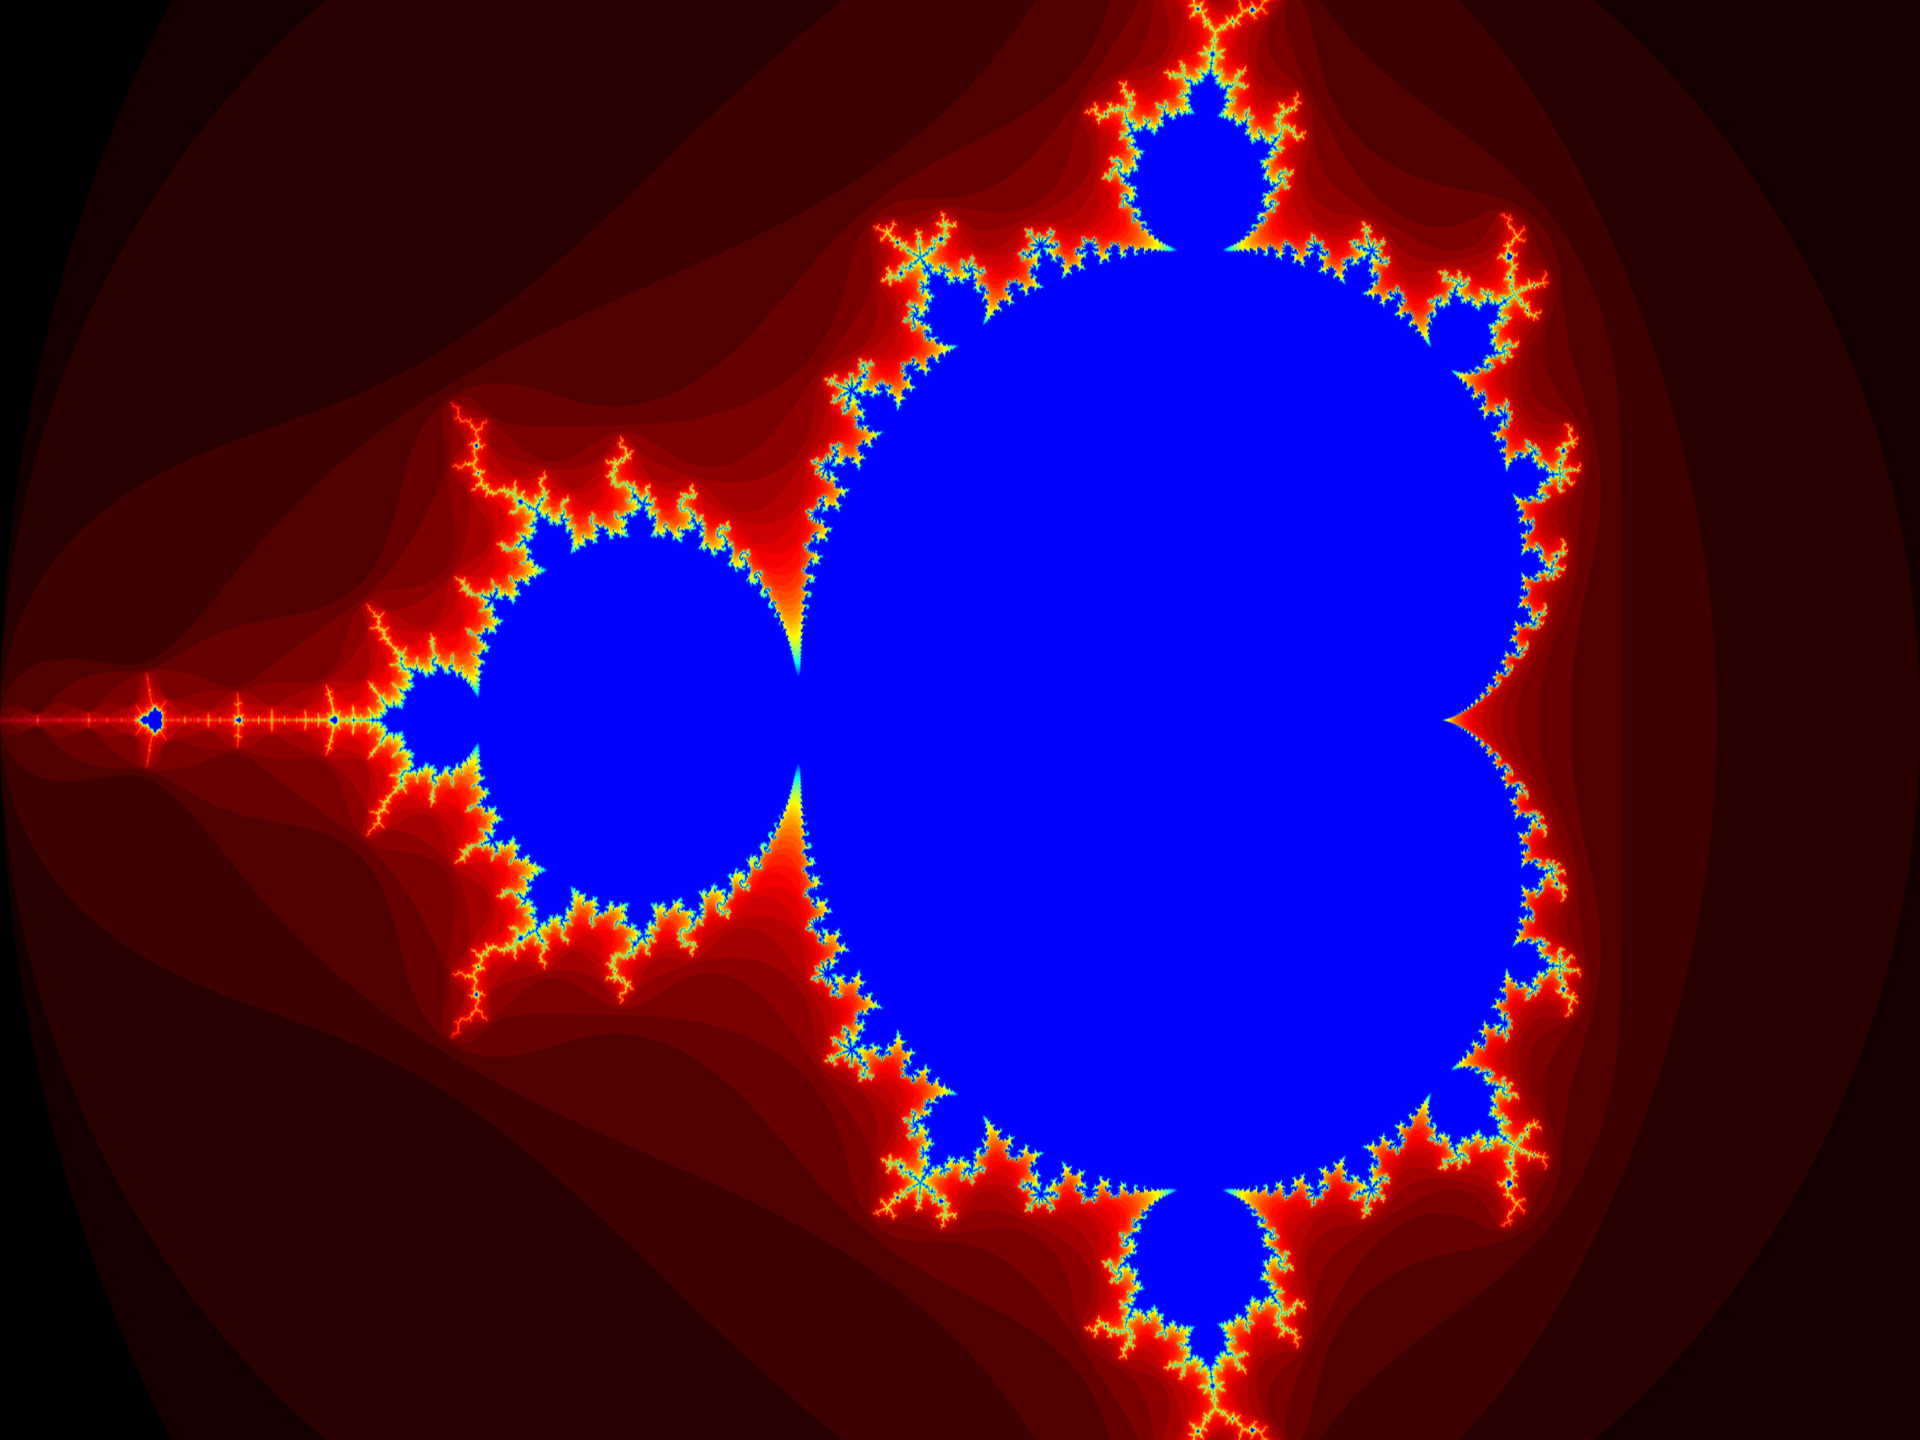
\includegraphics[width=\textwidth]{figures/comparacao/mandelbrot_50.png}
        \caption*{Imagem com 50 iterações}
    \end{minipage}
    \caption{Comparação entre imagens geradas com diferentes números de iterações.}
    \label{fig:comparison_iterations}
\end{figure}

As áreas pretas nas imagens geradas representam os pontos que não pertencem ao conjunto de Mandelbrot. Essas regiões indicam os valores no plano complexo onde a sequência iterativa diverge, ou seja, cresce sem limites após um grande número de iterações. Essa característica é fundamental para identificar as fronteiras complexas e os padrões intrincados que definem o conjunto.

\subsection{Intervalo do Plano Complexo}

O plano complexo foi definido com os seguintes limites:
\[
x \in [-2, 1], \quad y \in [-1, 1]
\]

Esse intervalo foi escolhido devido ao fato de que, para o conjunto de Mandelbrot, os valores de \( z \) que pertencem ao conjunto estão limitados a \( |z| \leq 2 \). Isso garante que a visualização esteja focada na região relevante do plano complexo, onde as iterações convergem e os padrões característicos do conjunto emergem.


\subsection{Kernel do Código e Tentativas de Otimização}

O núcleo do cálculo do conjunto de Mandelbrot é implementado na função \texttt{mandel}\cite{intel-fractal-code}, que realiza as iterações necessárias para determinar se um ponto no plano complexo pertence ao conjunto. A função utiliza a seguinte lógica:

\begin{lstlisting}[caption=Kernel do cálculo do conjunto de Mandelbrot]
static inline int mandel(float c_re, float c_im, int count)
{
    float z_re = c_re, z_im = c_im;
    float prev_mag_sq = z_re * z_re + z_im * z_im;
    int i;
    for (i = 0; i < count; ++i) {

        float mag_sq = z_re * z_re + z_im * z_im;

        if (mag_sq > 4.f)
            break;

        float new_re = z_re * z_re - z_im * z_im;
        float new_im = 2.f * z_re * z_im;
        z_re = c_re + new_re;
        z_im = c_im + new_im;

        prev_mag_sq = mag_sq;
    }

    return i;
}
\end{lstlisting}

Durante o desenvolvimento, foram realizadas tentativas de otimização para encontrar os pontos fixos, porém devido ao float, não consegui encontrar um intervalo de erro que conseguia parar a execução antes e encontrei imagens distorcidas.

Abaixo, apresentamos um exemplo de imagem gerada com a tentativa de otimização tentando encontrar pontos fixos, basta comparar com \autoref{fig:comparison_iterations} para ver as distorções introduzidas por isso:
\begin{figure}[H]
    \centering
    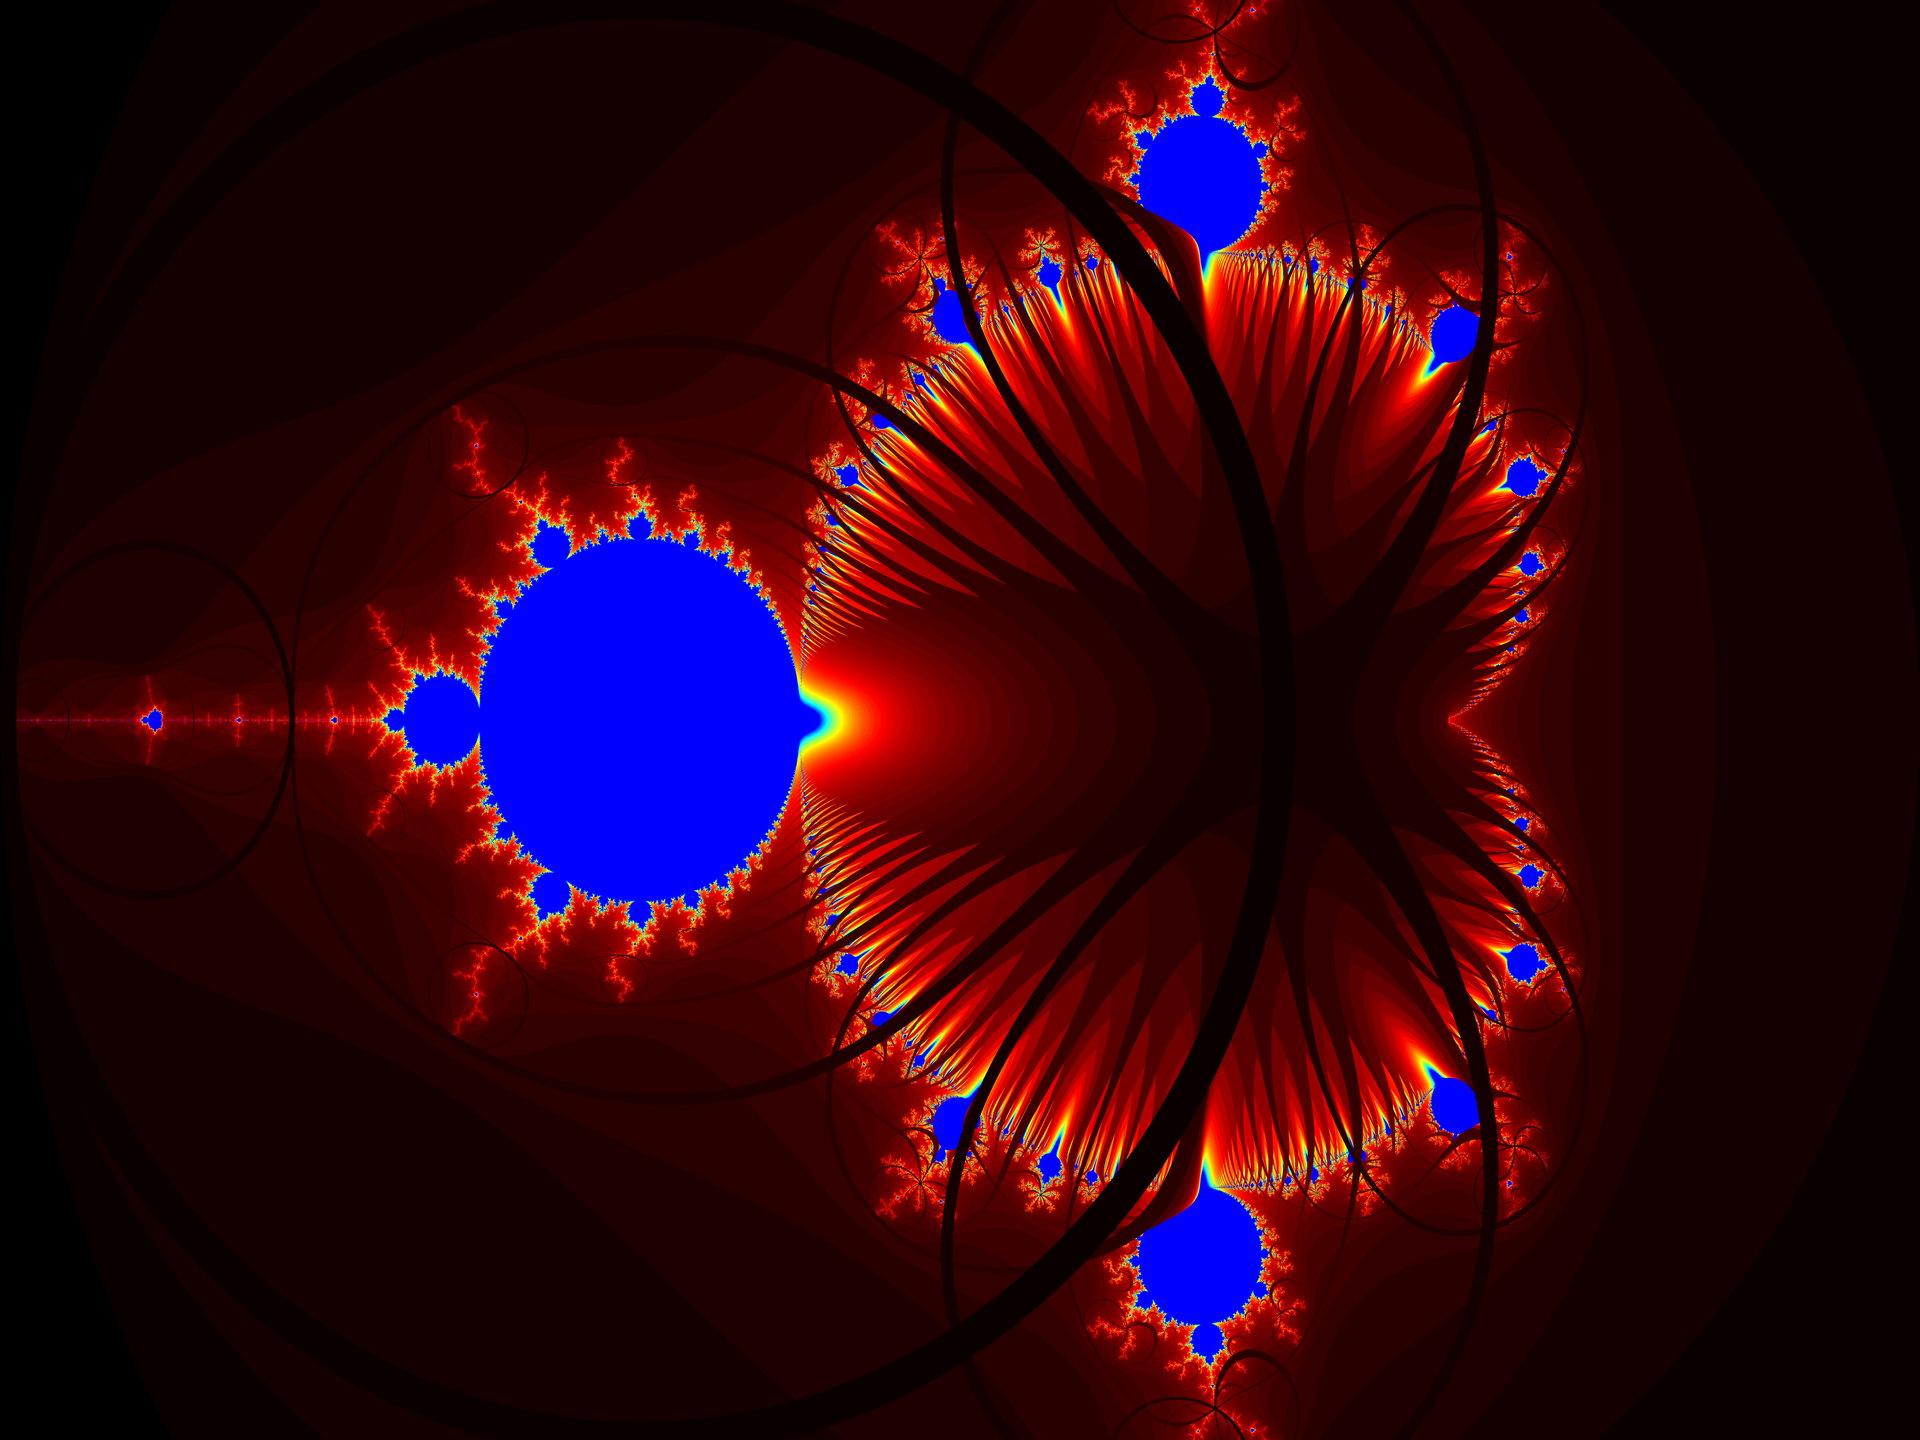
\includegraphics[width=0.7\textwidth]{figures/comparacao/mandelbrot_float.png}
    \caption{Imagem gerada com ponto flutuante.}
    \label{fig:comparison_float}
\end{figure}

Como resultado, a abordagem de encontrar pontos fixos foi descartada para preservar a qualidade das imagens geradas.
\subsection{Paralelismo}

A paralelização é feita utilizando múltiplas threads, controladas pelo parâmetro \texttt{--threads}. Cada thread é responsável por calcular uma fatia da imagem, dividida por linhas. O número de threads pode ser ajustado conforme o número de núcleos disponíveis na máquina.

Devido à alta resolução da imagem (\( 15360 \times 8640 \)) e ao elevado número de iterações (\( 10.000 \)), o tempo de execução ainda pode ser significativo, mesmo com paralelismo. Isso ocorre porque o cálculo de cada ponto no conjunto de Mandelbrot é computacionalmente intensivo, especialmente nas regiões de fronteira, onde a convergência é mais lenta e exige mais iterações para determinar se o ponto pertence ao conjunto. Além disso, a sobrecarga de criação e gerenciamento de threads também contribui para o tempo total de execução.
